% =====================================================================
% KidneyMTL -- 4-page IEEE conference paper (single file, compiles on Overleaf
% with pdfLaTeX; no external figures or .bib needed).
%
% STATUS: every red "??" (\tbd) and every red sentence (\finding{...}) depends on
% training results that do not exist yet (plan "paper_3folds" in the Colab
% notebook). All black numbers are final: they come from the data audit
% (data/splits/leakage_report.json), the dataset files and the parameter counts.
% GFLOPs/latency are re-measured at the v2 input sizes by notebook cell 5.2. Before submission: no red text may remain, and the reference
% list must be checked against the publisher pages.
% =====================================================================
\documentclass[conference]{IEEEtran}
\IEEEoverridecommandlockouts
\usepackage{cite}
\usepackage{amsmath,amssymb}
\usepackage{graphicx}
\usepackage{booktabs}
\usepackage{multirow}
\usepackage{xcolor}
\usepackage{tikz}
\usetikzlibrary{positioning,arrows.meta,fit}
\usepackage[hidelinks]{hyperref}

\newcommand{\tbd}{\textcolor{red}{\textbf{??}}}            % number pending
\newcommand{\finding}[1]{\textcolor{red}{#1}}             % sentence pending

\begin{document}

\title{Beyond Leaky Benchmarks: Leakage-Aware Multi-Task Learning for Kidney Disease Classification and Stone Localisation in CT}

\author{\IEEEauthorblockN{Utkarsh Kumar, Koynaa Jain, Unmukt Gupta, Neil Sanghvi}
\IEEEauthorblockA{Manipal Institute of Technology Bengaluru,\\
Manipal Academy of Higher Education, Manipal, India\\
utkarsh2.mitblr2024@learner.manipal.edu, koynaa.mitblr2024@learner.manipal.edu,\\
unmukt.mitblr2024@learner.manipal.edu, neil.mitblr2024@learner.manipal.edu}}

\maketitle

% ---------------------------------------------------------------------
\begin{abstract}
Deep-learning studies on the public CT-KIDNEY dataset routinely report accuracies above 99\%. We show that
much of this performance comes from the evaluation protocol rather than from the models. A perceptual-hash audit
of the 12,446 slices finds 517 sets of byte-identical files and shows that 99.3\% of test images in a random
image-level split have a near-duplicate (Hamming distance $\le$4 of 64 bits) in the training set; augmenting
the data before splitting, as done in recent work, places transformed copies of 98.6\% of the test images in the
training set. We propose (i) a leakage-aware protocol that keeps every group of near-duplicate slices inside one
fold, and (ii) KidneyMTL, a compact multi-task network (11.2M parameters) that learns four-class kidney
classification (normal, cyst, stone, tumour) and anchor-free stone localisation from two partially labelled
datasets, using a tri-channel CT/CLAHE/contour input, CBAM attention and bounded uncertainty-based task
weighting. Under the grouped protocol KidneyMTL reaches a macro-F1 of \tbd\% and a stone-detection mAP@0.5 of
\tbd\%, against \tbd\% for a re-implementation of the recent CDR-VGG19 model (142M parameters). Re-training the
same baselines under the random and augment-then-split protocols inflates macro-F1 by up to \tbd{} points. Code
and fold assignments are publicly available.
\end{abstract}

\begin{IEEEkeywords}
kidney stone, computed tomography, data leakage, multi-task learning, object detection, model evaluation
\end{IEEEkeywords}

% ---------------------------------------------------------------------
\section{Introduction}
Non-contrast CT is the reference imaging test for kidney stones. Cysts and renal tumours appear on the same
scans, so an automated reader should separate these conditions and, for stones, show \emph{where} the stone is.
Most recent deep-learning work treats the task as image-level classification on public datasets and reports
accuracies between 98\% and 99.9\%~\cite{islam2022vision,devi2025cdr,yildirim2021deep}.

Two problems make these numbers hard to interpret. First, the widely used CT-KIDNEY dataset~\cite{islam2022vision}
contains no patient identifiers and consists of consecutive, highly similar slices, so a random image-level split
puts near-copies of each test image into the training set. Second, some studies augment the data
\emph{before} splitting it (21 variants per image in~\cite{devi2025cdr}), so rotated or flipped copies of a test
image are seen during training. Both are forms of data leakage, a documented cause of irreproducible results in
machine learning and medical imaging~\cite{kapoor2023leakage,roberts2021pitfalls,varoquaux2022failures}.
In addition, almost all prior models output only a class label, although localising the stone is more useful
clinically and allows checking whether the decision relies on the lesion.

Our contributions are:
(1)~a near-duplicate audit of CT-KIDNEY and a grouped, stratified cross-validation protocol free of
near-duplicate leakage;
(2)~a controlled experiment that re-trains identical models under grouped, random and augment-then-split
protocols and measures the resulting inflation;
(3)~KidneyMTL, a multi-task network trained on two partially labelled datasets that classifies kidney CT
slices and localises stones, with a bounded variant of uncertainty task weighting that avoids a weight
blow-up we observed with the original formulation.

% ---------------------------------------------------------------------
\section{Related Work}
Islam et al.~\cite{islam2022vision} released CT-KIDNEY and reported 99.3\% accuracy with a Swin transformer
under a random split. Devi et al.~\cite{devi2025cdr} feed contour-detected images to a VGG-19 with a normalised
residual block (CDR-VGG19) and report 99.61\% accuracy after 21$\times$ augmentation followed by an
80:10:10 split. Yildirim et al.~\cite{yildirim2021deep} classify coronal CT images as stone or normal, while
Parakh et al.~\cite{parakh2019urinary} and Elton et al.~\cite{elton2022deep} detect and segment stones on
volumetric CT. Kendall et al.~\cite{kendall2018multi} weight multi-task losses by learned homoscedastic
uncertainty. Roberts et al.~\cite{roberts2021pitfalls} attributed the failure of most COVID-19 imaging models
partly to duplicated data, and Kapoor and Narayanan~\cite{kapoor2023leakage} list leakage across scientific
fields. To our knowledge, no prior work has quantified leakage on CT-KIDNEY.

% ---------------------------------------------------------------------
\section{Data and Leakage-Aware Protocol}\label{sec:protocol}
\textbf{Classification data.} CT-KIDNEY~\cite{islam2022vision} has 12,446 axial CT slices: Normal (5,077),
Cyst (3,709), Tumour (2,283) and Stone (1,377).
\textbf{Localisation data.} A public box-annotated kidney-stone dataset of coronal CT images (Roboflow export
of the data of~\cite{yildirim2021deep}) with 1,054/123/123 train/validation/test images and 2,278/325/224 stone
boxes. We verified that no source image crosses its splits. It has no non-stone classes, and CT-KIDNEY has no
boxes, so neither dataset alone supports joint training.

\textbf{Near-duplicate audit.} We compute a 64-bit DCT perceptual hash~\cite{zauner2010phash} of every slice
and link slices whose Hamming distance is $\le\tau$. Connected components form groups. With $\tau{=}4$ the data
form 229 groups (largest 705 slices). Larger thresholds chain almost half the dataset into one component, so
$\tau{=}4$ is the strictest threshold that still yields usable folds. Table~\ref{tab:audit} shows that a random
split places a near-identical copy of almost every test slice in the training set (median nearest-neighbour
distance 0 bits).

\begin{table}[t]
\centering
\caption{Near-duplicate audit of CT-KIDNEY (5-fold mean). NN: nearest training image of each test image
(64-bit pHash).}
\label{tab:audit}
\setlength{\tabcolsep}{4pt}
\begin{tabular}{lcc}
\toprule
Protocol & Test with NN $\le$4 bits & Median NN dist. \\
\midrule
Random image split & 99.3\% & 0.0 \\
Augment-then-split~\cite{devi2025cdr} & 98.6\%$^\dagger$ & -- \\
Grouped (ours) & \textbf{0.0\%} & \textbf{10.4} \\
\bottomrule
\multicolumn{3}{l}{\footnotesize $^\dagger$Test source images with an augmented copy in training.}\\
\multicolumn{3}{l}{\footnotesize Byte-identical file sets: 517 (1,034 images).}
\end{tabular}
\end{table}

\textbf{Protocol.} Groups are distributed over five parts with stratified group $k$-fold. In fold $k$, part $k$ is
the test set, part $(k{+}1)\bmod 5$ is the validation set (model selection, early stopping) and the remaining
three parts form the training set, so every slice is tested once. For the leakage experiment we also build a
stratified \emph{random} image-level split and the \emph{augment-then-split} protocol of~\cite{devi2025cdr}: each
image is expanded into five deterministic variants (rotations, flips, intensity changes, noise, zoom) that are
then split at random. Using five instead of 21 variants yields fewer leaked copies, so the inflation we measure
is, if anything, an underestimate. To give all protocols the same optimisation budget, augment-then-split
training is capped at the number of steps per epoch of the grouped protocol (233).

% ---------------------------------------------------------------------
\section{KidneyMTL}\label{sec:method}
\begin{figure}[t]
\centering
\resizebox{\columnwidth}{!}{%
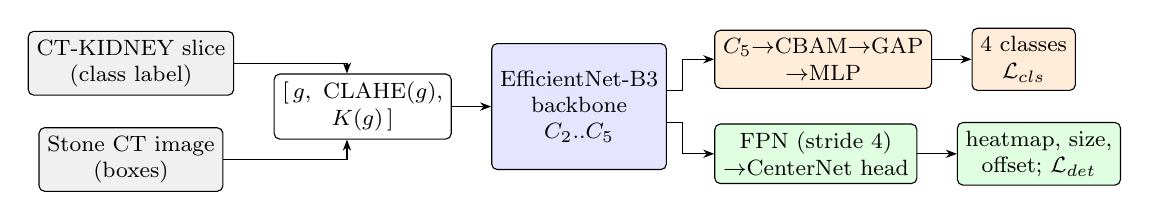
\begin{tikzpicture}[
  font=\footnotesize, >={Stealth[length=4pt]},
  box/.style={draw, rounded corners=2pt, align=center, minimum height=7mm, inner sep=3pt},
  data/.style={box, fill=gray!12},
  net/.style={box, fill=blue!10},
  cls/.style={box, fill=orange!15},
  det/.style={box, fill=green!12}]
  \node[data] (ck) {CT-KIDNEY slice\\(class label)};
  \node[data, below=4mm of ck] (sd) {Stone CT image\\(boxes)};
  \node[box, right=5mm of ck, yshift=-5.5mm] (inp) {$[\,g,\ \mathrm{CLAHE}(g),$\\$K(g)\,]$};
  \node[net, right=5mm of inp, minimum height=16mm] (bb) {EfficientNet-B3\\backbone\\$C_2..C_5$};
  \node[cls, right=6mm of bb, yshift=6mm] (cbam) {$C_5$$\rightarrow$CBAM$\rightarrow$GAP\\$\rightarrow$MLP};
  \node[det, right=6mm of bb, yshift=-6mm] (fpn) {FPN (stride 4)\\$\rightarrow$CenterNet head};
  \node[cls, right=5mm of cbam] (yc) {4 classes\\$\mathcal{L}_{cls}$};
  \node[det, right=5mm of fpn] (yd) {heatmap, size,\\offset; $\mathcal{L}_{det}$};
  \draw[->] (ck) -| ([xshift=-2mm]inp.north);
  \draw[->] (sd) -| ([xshift=-2mm]inp.south);
  \draw[->] (inp) -- (bb);
  \draw[->] (bb.east) ++(0,2mm) -- ++(2mm,0) |- (cbam.west);
  \draw[->] (bb.east) ++(0,-2mm) -- ++(2mm,0) |- (fpn.west);
  \draw[->] (cbam) -- (yc);
  \draw[->] (fpn) -- (yd);
\end{tikzpicture}}
\caption{KidneyMTL. Each step draws one classification batch and one localisation batch; the shared backbone
is updated with $e^{-s_c}\mathcal{L}_{cls}+s_c+e^{-s_d}\mathcal{L}_{det}+s_d$, with bounded $s_c,s_d$.}
\label{fig:arch}
\end{figure}

\textbf{Input.} Each grey-level slice $g$ becomes three channels $[\,g,\ \mathrm{CLAHE}(g),\ K(g)\,]$, where
$K(g)$ is a multi-level iso-intensity contour map: after Gaussian smoothing, contours are traced at the Otsu
threshold and at the 85th, 95th and 99th foreground intensity percentiles, so hyper-dense stones receive nested
high-level contours. Unlike~\cite{devi2025cdr}, the contour map is added to the image, not substituted for it.

\textbf{Architecture} (Fig.~\ref{fig:arch}). An ImageNet-pretrained EfficientNet-B3~\cite{tan2019efficientnet}
provides features at strides 4--32. The classification head applies CBAM~\cite{woo2018cbam}, global average
pooling, dropout, a 256-unit SiLU layer and a linear layer. The localisation branch fuses all levels with a
top-down FPN~\cite{lin2017fpn} into a 128-channel stride-4 map and applies a CenterNet head~\cite{zhou2019objects}
that predicts a stone-centre heatmap, box size and sub-pixel offset. Boxes are decoded with $3{\times}3$
max-pooling and the top-50 peaks.

\textbf{Losses.} Classification uses the focal loss~\cite{lin2017focal} ($\gamma{=}2$) with
inverse-square-root class weights and label smoothing 0.05. Localisation uses
$\mathcal{L}_{det}=\mathcal{L}_{hm}+\mathcal{L}_{off}+2\,\mathcal{L}_{CIoU}$: the penalty-reduced focal
heatmap loss, an $L_1$ offset loss and the CIoU loss~\cite{zheng2020diou}.

\textbf{Bounded uncertainty weighting.} With $\mathcal{L}=\sum_i e^{-s_i}\mathcal{L}_i+s_i$~\cite{kendall2018multi}
the optimum is $s_i=\log\mathcal{L}_i$. A task whose training loss approaches zero therefore receives an unbounded
weight, which effectively raises its learning rate without limit. In a preliminary run, the classification
weight $e^{-s_c}$ rose from 1 to 44 within 20 epochs while its training loss fell below $10^{-3}$, and
validation accuracy oscillated between 85\% and 91\%. We therefore project $s_i$ onto $[-1,3]$ after every
optimiser step, which limits task weights to $[0.05,\,2.72]$.

\textbf{Partially labelled training.} Every step combines one CT-KIDNEY batch (32 slices, $256^2$,
classification loss only) with one stone batch (8 images letterboxed to $384^2$, i.e.\ their native
$320{\times}391$ resolution, localisation loss only). No image needs both kinds of label.

% ---------------------------------------------------------------------
\section{Experimental Setup}
\textbf{Models.} We compare KidneyMTL with (a) the same network without the localisation task (single-task
ablation), (b) ResNet-50~\cite{he2016resnet} fine-tuned with cross-entropy on grey-level input, the standard
practice, and (c) CDR-VGG19~\cite{devi2025cdr}, re-implemented from its description (VGG-19~\cite{simonyan2015vgg},
two 4096-unit layers, a 4096-320-320-4096 normalised residual block and $224^2$ contour input).
\textbf{Training.} AdamW (backbone learning rate $2{\times}10^{-4}$, heads $10^{-3}$), 1-epoch warm-up and cosine
decay, at most 12 epochs with early stopping on validation macro-F1 (patience 4), mixed precision, an
exponential moving average of the weights and horizontal-flip test-time augmentation. For augment-then-split,
models are selected on the original validation images and tested on all variants. Online augmentation:
flips, affine transforms, brightness/contrast, gamma, noise, blur and coarse dropout. All models share the
augmentation, schedule and folds. Experiments ran on an NVIDIA T4 (16\,GB) with PyTorch~2 and timm~1.0.15.
For budget reasons we report the first three of the five folds (7,457/2,485/2,504 train/val./test slices in fold 0).
\textbf{Metrics.} Accuracy, macro-F1, macro one-vs-rest AUC, stone-vs-rest sensitivity and expected calibration
error (ECE, 15 bins)~\cite{guo2017calibration}, given as mean$\pm$s.d.\ over test folds. Confidence intervals
(95\%) use a cluster bootstrap that resamples whole near-duplicate groups (2,000 replicates). Paired comparisons
use exact McNemar tests with Holm correction. Localisation is measured by COCO-style AP at IoU 0.5 and
0.5:0.95.

% ---------------------------------------------------------------------
\section{Results}
\subsection{How much does the protocol inflate performance?}
\begin{table}[t]
\centering
\caption{Accuracy / macro-F1 (\%) of identical models under three protocols (3 folds). The gap to the grouped
protocol is the inflation caused by leakage.}
\label{tab:leakage}
\small\setlength{\tabcolsep}{3pt}
\begin{tabular}{lccc}
\toprule
Model & Grouped (ours) & Random split & Aug.-then-split \\
\midrule
ResNet-50 & \tbd{} / \tbd & \tbd{} / \tbd & \tbd{} / \tbd \\
CDR-VGG19 & \tbd{} / \tbd & \tbd{} / \tbd & \tbd{} / \tbd \\
\midrule
CDR-VGG19, published~\cite{devi2025cdr} & -- & -- & 99.61 / -- \\
\bottomrule
\end{tabular}
\end{table}

Table~\ref{tab:leakage} shows the same architectures trained and tested under each protocol.
\finding{Under the random and augment-then-split protocols both models approach the near-perfect accuracies
reported in the literature (\tbd\% for our CDR-VGG19 re-implementation versus 99.61\% published), whereas the
grouped protocol lowers macro-F1 by \tbd{} (ResNet-50) and \tbd{} points (CDR-VGG19).} The gap is largest for
the augment-then-split protocol, \finding{consistent with} the audit in Table~\ref{tab:audit}: almost every test
image has a training copy that differs only by a geometric or intensity transform.

\subsection{Comparison under the leakage-free protocol}
\begin{table*}[t]
\centering
\caption{Grouped 3-fold cross-validation on CT-KIDNEY (mean$\pm$s.d., \%). Parameters and FLOPs are for the
classification path at the stated input size; latency is batch-1 median on an NVIDIA T4. $^\ast$McNemar
$p<0.05$ against KidneyMTL after Holm correction.}
\label{tab:main}
\small\setlength{\tabcolsep}{4pt}
\begin{tabular}{lccccccccc}
\toprule
Model & Input & Params (M) & GFLOPs & Latency (ms) & Accuracy & Macro-F1 & Macro AUC & Stone sens. & ECE $\downarrow$ \\
\midrule
ResNet-50~\cite{he2016resnet} & $256^2$ gray & 23.5 & \tbd & \tbd & \tbd & \tbd & \tbd & \tbd & \tbd \\
CDR-VGG19~\cite{devi2025cdr} (re-impl.) & $224^2$ contour & 142.3 & 39.26 & \tbd & \tbd & \tbd & \tbd & \tbd & \tbd \\
KidneyMTL w/o localisation & $256^2$ tri & 10.2 & \tbd & \tbd & \tbd & \tbd & \tbd & \tbd & \tbd \\
\textbf{KidneyMTL (ours)} & $256^2$ tri & 10.2$^\dagger$ & \tbd & \tbd & \tbd & \tbd & \tbd & \tbd & \tbd \\
\bottomrule
\multicolumn{10}{l}{\footnotesize $^\dagger$11.2M including the localisation branch (\tbd{} GFLOPs, \tbd\,ms at $384^2$), which is not needed for classification.}
\end{tabular}
\end{table*}

Table~\ref{tab:main} compares the models under the grouped protocol.
\finding{KidneyMTL achieves the highest macro-F1 (\tbd\%, 95\% CI [\tbd, \tbd]) with 14$\times$ fewer parameters
and \tbd$\times$ fewer FLOPs than CDR-VGG19.} \finding{Removing the localisation task changes macro-F1 by \tbd{}
points and stone sensitivity by \tbd{} points}, which isolates the effect of multi-task training on
classification. \finding{The most frequent error of all models is tumour slices predicted as normal}, reflecting
the low contrast of small renal masses on JPEG-compressed slices. \finding{KidneyMTL is also the best calibrated
model (ECE \tbd\%), which matters when probabilities are used for triage.}

\subsection{Stone localisation, explainability and transfer}
\begin{table}[t]
\centering
\caption{Stone localisation on the held-out coronal test split (123 images, 224 stones) and cross-dataset
behaviour of KidneyMTL (mean over 3 runs).}
\label{tab:det}
\small\setlength{\tabcolsep}{4pt}
\begin{tabular}{lc}
\toprule
mAP@0.5 / mAP@0.5:0.95 & \tbd{} / \tbd \\
Precision / recall @0.5 (score $\ge$0.3) & \tbd{} / \tbd \\
Images with $\ge$1 correctly found stone & \tbd \\
\midrule
Pointing game: Grad-CAM~\cite{selvaraju2017gradcam} / detection heatmap & \tbd{} / \tbd \\
Coronal test images classified as Stone & \tbd \\
\bottomrule
\end{tabular}
\end{table}

Table~\ref{tab:det} reports localisation, which no classification-only model provides.
\finding{KidneyMTL localises \tbd\% of stones at IoU 0.5; most misses are small stones of a few pixels, which
explains the lower mAP@0.5:0.95.} The pointing game~\cite{zhang2016topdown} measures whether the maximum of a
saliency map falls inside an annotated stone. \finding{The detection heatmap points at a stone in \tbd\% of
images, whereas the Grad-CAM map of the classification head does so in only \tbd\%}: class-activation maps
are a poor proxy for lesion localisation, and an explicit localisation output is the more reliable
explanation. Finally, the classifier, trained only on axial slices, \finding{labels \tbd\% of the unseen coronal
stone images as Stone}. This cross-view shift shows that high in-distribution accuracy does not by itself imply
generalisation.

% ---------------------------------------------------------------------
\section{Discussion and Limitations}
Our results indicate that published near-perfect accuracies on CT-KIDNEY \finding{largely} measure recognition of
near-duplicate slices. We recommend that future studies split by patient or, when no identifiers exist, by
near-duplicate group, never augment before splitting, and release their fold assignments. Hash groups only
approximate patients: 14 of the 229 groups contain more than one class, and distant slices of one patient may
fall into different groups, so the grouped protocol removes near-duplicate leakage but does not guarantee
patient-level independence. Further limitations are the use of 2D JPEG slices without Hounsfield units, a single
public source per task, the axial/coronal mismatch between the two datasets, the reporting of three of five
folds, and the absence of a reader study. Future work will use volumetric multi-centre DICOM data with patient
identifiers.

\section{Conclusion}
We showed that standard evaluation protocols on CT-KIDNEY leak near-duplicate slices into the test set and
inflate reported performance \finding{by up to \tbd{} macro-F1 points}. Under a leakage-free grouped protocol,
KidneyMTL, a compact multi-task network with bounded uncertainty weighting, \finding{classifies kidney CT slices
with a macro-F1 of \tbd\% while also localising stones (mAP@0.5 \tbd\%)} at a fraction of the cost of recent
models. Code, configurations and fold assignments are available at
\url{https://github.com/utkarshhzz/Kidney_research}.

% ---------------------------------------------------------------------
\begin{thebibliography}{99}
\footnotesize

\bibitem{islam2022vision}
M.~N. Islam, M.~Hasan, M.~K. Hossain, M.~G.~R. Alam, M.~Z. Uddin, and A.~Soylu, ``Vision transformer and
explainable transfer learning models for auto detection of kidney cyst, stone and tumor from CT-radiography,''
\emph{Sci. Rep.}, vol.~12, Art.~no.~11440, 2022.

\bibitem{devi2025cdr}
S.~Devi~M., Y.~Natarajan, P.~S., and S.~P.~K.~R., ``Contour-detected normalized residual model for kidney stone
classification,'' \emph{Appl. Comput. Intell. Soft Comput.}, vol.~2025, Art.~no.~5844438, 2025.

\bibitem{yildirim2021deep}
K.~Yildirim, P.~G. Bozdag, M.~Talo, O.~Yildirim, M.~Karabatak, and U.~R. Acharya, ``Deep learning model for
automated kidney stone detection using coronal CT images,'' \emph{Comput. Biol. Med.}, vol.~135, Art.~no.~104569,
2021.

\bibitem{kapoor2023leakage}
S.~Kapoor and A.~Narayanan, ``Leakage and the reproducibility crisis in machine-learning-based science,''
\emph{Patterns}, vol.~4, no.~9, Art.~no.~100804, 2023.

\bibitem{roberts2021pitfalls}
M.~Roberts \emph{et al.}, ``Common pitfalls and recommendations for using machine learning to detect and
prognosticate for COVID-19 using chest radiographs and CT scans,'' \emph{Nat. Mach. Intell.}, vol.~3,
pp.~199--217, 2021.

\bibitem{varoquaux2022failures}
G.~Varoquaux and V.~Cheplygina, ``Machine learning for medical imaging: methodological failures and
recommendations for the future,'' \emph{npj Digit. Med.}, vol.~5, Art.~no.~48, 2022.

\bibitem{parakh2019urinary}
A.~Parakh \emph{et al.}, ``Urinary stone detection on CT images using deep convolutional neural networks:
evaluation of model performance and generalization,'' \emph{Radiol. Artif. Intell.}, vol.~1, no.~4,
Art.~no.~e180066, 2019.

\bibitem{elton2022deep}
D.~C. Elton, E.~B. Turkbey, P.~J. Pickhardt, and R.~M. Summers, ``A deep learning system for automated kidney
stone detection and volumetric segmentation on noncontrast CT scans,'' \emph{Med. Phys.}, vol.~49, no.~4,
pp.~2545--2554, 2022.

\bibitem{kendall2018multi}
A.~Kendall, Y.~Gal, and R.~Cipolla, ``Multi-task learning using uncertainty to weigh losses for scene geometry
and semantics,'' in \emph{Proc. IEEE CVPR}, 2018, pp.~7482--7491.

\bibitem{zauner2010phash}
C.~Zauner, ``Implementation and benchmarking of perceptual image hash functions,'' M.S. thesis, Upper Austria
Univ. Appl. Sci., Hagenberg, Austria, 2010.

\bibitem{tan2019efficientnet}
M.~Tan and Q.~Le, ``EfficientNet: Rethinking model scaling for convolutional neural networks,'' in
\emph{Proc. ICML}, 2019, pp.~6105--6114.

\bibitem{woo2018cbam}
S.~Woo, J.~Park, J.-Y. Lee, and I.~S. Kweon, ``CBAM: Convolutional block attention module,'' in
\emph{Proc. ECCV}, 2018, pp.~3--19.

\bibitem{lin2017fpn}
T.-Y. Lin, P.~Doll\'ar, R.~Girshick, K.~He, B.~Hariharan, and S.~Belongie, ``Feature pyramid networks for
object detection,'' in \emph{Proc. IEEE CVPR}, 2017, pp.~2117--2125.

\bibitem{zhou2019objects}
X.~Zhou, D.~Wang, and P.~Kr\"ahenb\"uhl, ``Objects as points,'' \emph{arXiv:1904.07850}, 2019.

\bibitem{lin2017focal}
T.-Y. Lin, P.~Goyal, R.~Girshick, K.~He, and P.~Doll\'ar, ``Focal loss for dense object detection,'' in
\emph{Proc. IEEE ICCV}, 2017, pp.~2980--2988.

\bibitem{zheng2020diou}
Z.~Zheng, P.~Wang, W.~Liu, J.~Li, R.~Ye, and D.~Ren, ``Distance-IoU loss: Faster and better learning for
bounding box regression,'' in \emph{Proc. AAAI}, vol.~34, 2020, pp.~12993--13000.

\bibitem{he2016resnet}
K.~He, X.~Zhang, S.~Ren, and J.~Sun, ``Deep residual learning for image recognition,'' in \emph{Proc. IEEE CVPR},
2016, pp.~770--778.

\bibitem{simonyan2015vgg}
K.~Simonyan and A.~Zisserman, ``Very deep convolutional networks for large-scale image recognition,'' in
\emph{Proc. ICLR}, 2015.

\bibitem{guo2017calibration}
C.~Guo, G.~Pleiss, Y.~Sun, and K.~Q. Weinberger, ``On calibration of modern neural networks,'' in
\emph{Proc. ICML}, 2017, pp.~1321--1330.

\bibitem{selvaraju2017gradcam}
R.~R. Selvaraju, M.~Cogswell, A.~Das, R.~Vedantam, D.~Parikh, and D.~Batra, ``Grad-CAM: Visual explanations from
deep networks via gradient-based localization,'' in \emph{Proc. IEEE ICCV}, 2017, pp.~618--626.

\bibitem{zhang2016topdown}
J.~Zhang, Z.~Lin, J.~Brandt, X.~Shen, and S.~Sclaroff, ``Top-down neural attention by excitation backprop,'' in
\emph{Proc. ECCV}, 2016, pp.~543--559.

\end{thebibliography}

\end{document}
